\subsection{Equilibrium results}
\label{subsec:monte_carlo_results}
First we look into relation between order parameter~\eqref{eq:nematic_order_parameter} and $k_BT$ at equilibrium for different system densities. As we can see on the Figure~\ref{fig:op_kbt}, the nematic order increases with decrease of $k_BT$. Black color shows results for $N = 6400$ and red color for $N = 1600$ particles. Lines show results obtained by means of Monte-Carlo simulations, and points are obtained from Langevin dynamics simulations allowed to equilibrate for $t = 500$. The results are average over $200$ samples. Important to observer rapid increase in order parameter in low temperature. The region of rapid increase shifts with densities, and for higher density the relation between order parameter and $k_BT$ closer to linear. As we can see, there is no systematic scaling with system size, and both MC and LD results are in good agreement.

\begin{figure}[h]
\centering
\begin{subfigure}[t]{0.49\textwidth}
	\centering
	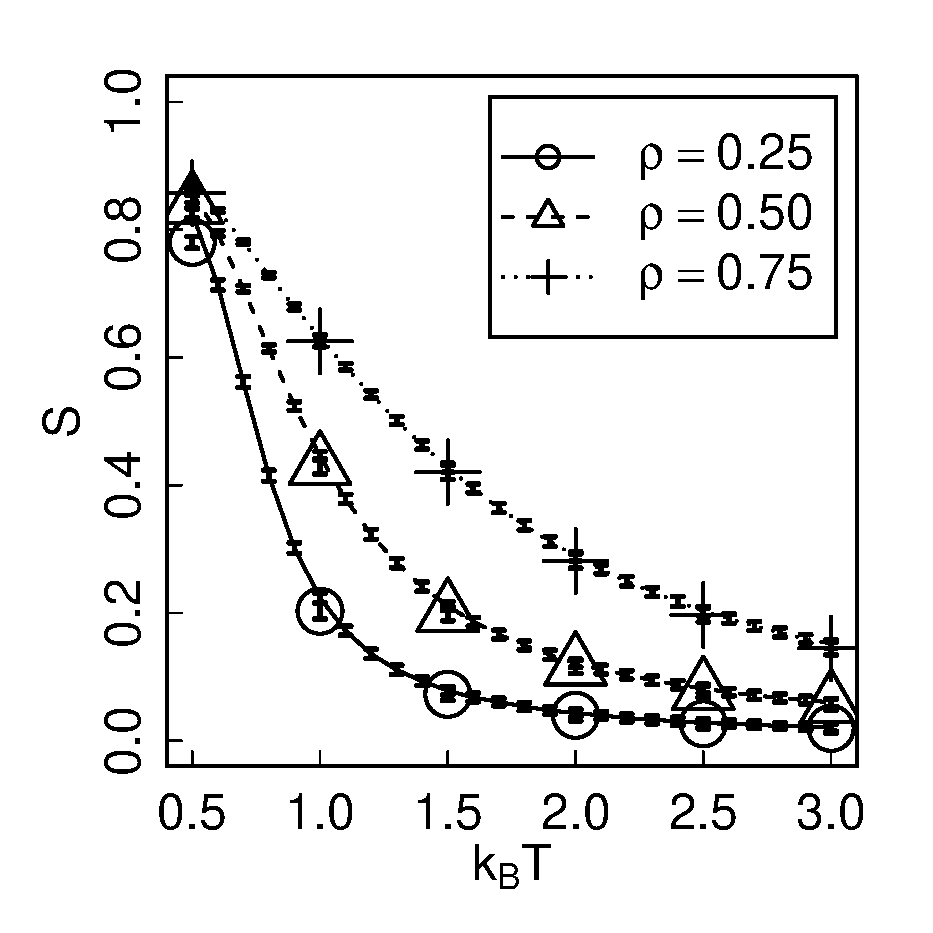
\includegraphics[width=\textwidth]{Images/op_eq_6400}
\end{subfigure}
\begin{subfigure}[t]{0.49\textwidth}
	\centering
	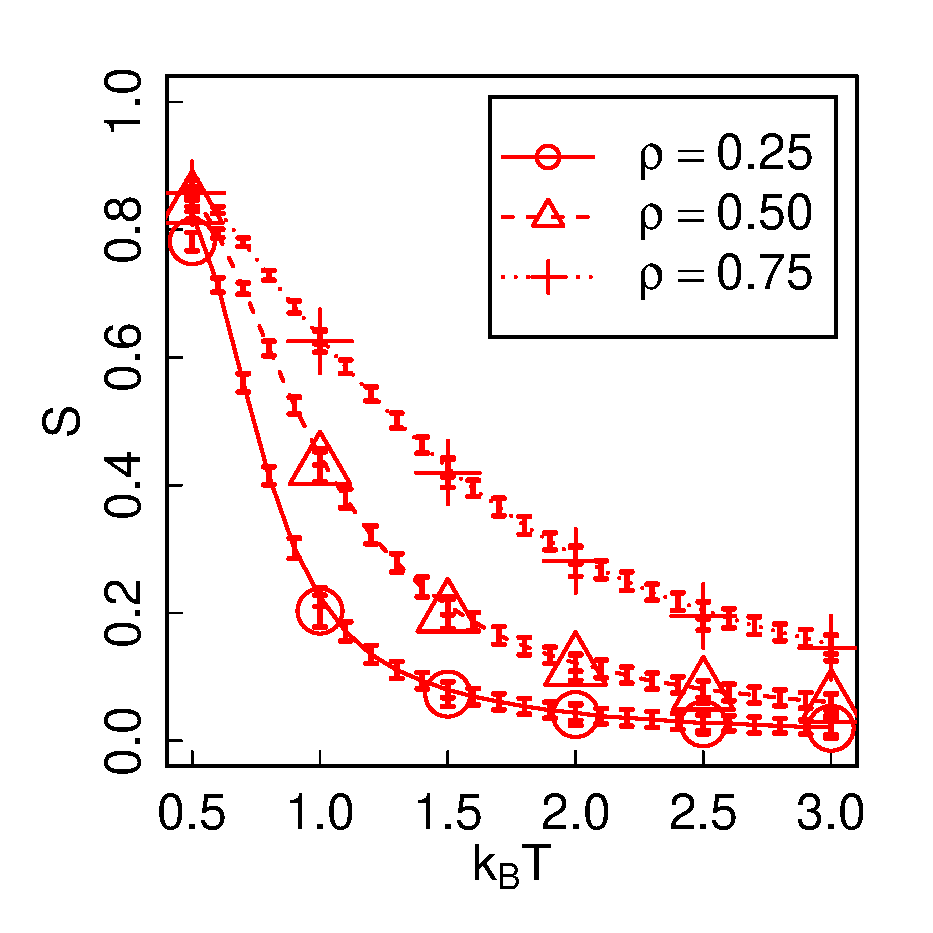
\includegraphics[width=\textwidth]{Images/op_eq_1600}
\end{subfigure}

	\captionsetup{justification=centering, width=0.9\columnwidth}
	\caption{Order parameter defined by eq.~\eqref{eq:nematic_order_parameter} versus $k_BT$ for Monte-Carlo simulations. Black color shows results for $N = 6400$ and red color for $N = 1600$ particles. As we can see there is no systematic scaling with system size. Lines show results obtained by means of MC simulations, and points are obtained from LD simulations at $t = 500$ starting from random initial configuration. The results are average over $200$ samples as described in sec.~\ref{subsec:simulation_details}}
	\label{fig:op_kbt}
\end{figure}

Growth of nematic order parameter with decrease of temperature may imply structural changes in observed system. To investigate that, we first calculate the probability of having two chains pointing in the same direction (along or counter $z$ axis) or in opposite directions for different $k_BT$.

Next we analyse the orientation correlation (i.e. the level of co-alignment) of particles as function of distance between them. For all observed range of simulation parameters the correlation (i.e. co-alignment between dipole moments of two particles) decays exponentially with distance. For selected number of simulation parameters the results are presented at the Figure \ref{fig:dist_corr_eq}, done in log-linear scale. The dots are obtained with space sampling $\delta = 1/6$, and are averaged over $200$ samples with $N = 6400$ particles. Lines are obtained by linear approximation of the results in range $0.01 < C(\Delta z) < 0.45$.
\begin{figure}[h]
\centering
\begin{subfigure}[t]{0.32\textwidth}
	\centering
	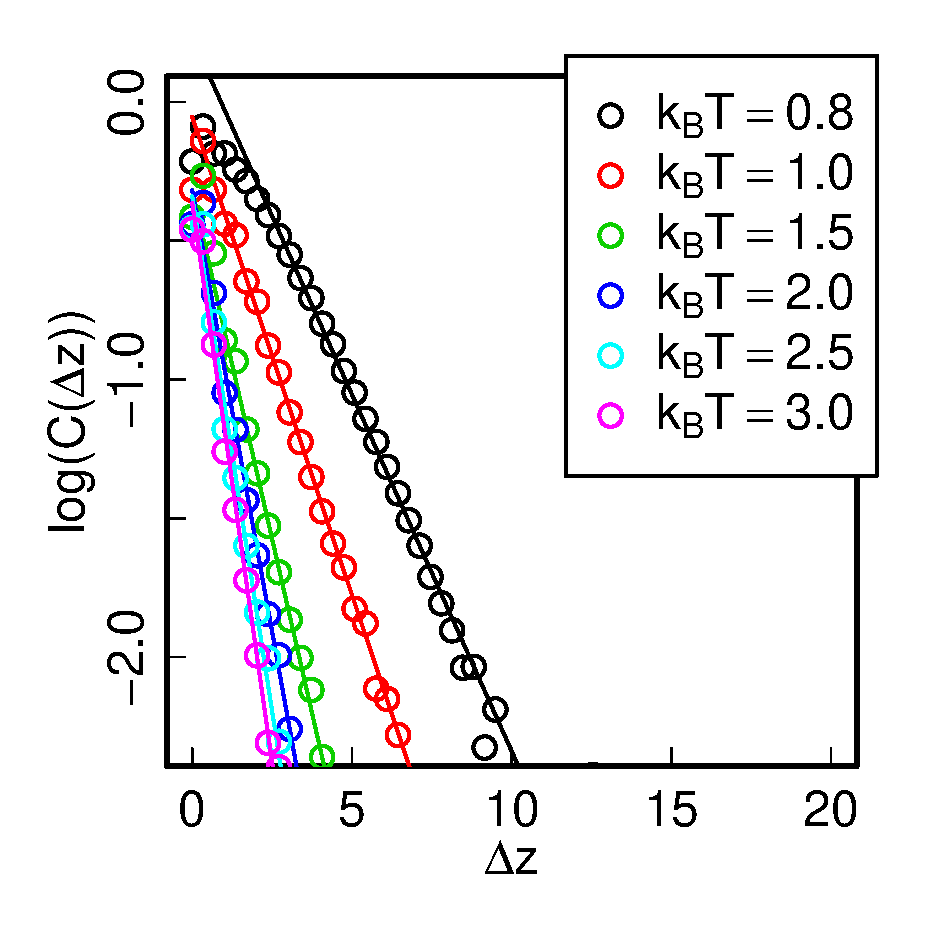
\includegraphics[width=\textwidth]{Images/distCor_25}
	\caption{$\rho = 0.25$}
\end{subfigure}
\begin{subfigure}[t]{0.32\textwidth}
	\centering
	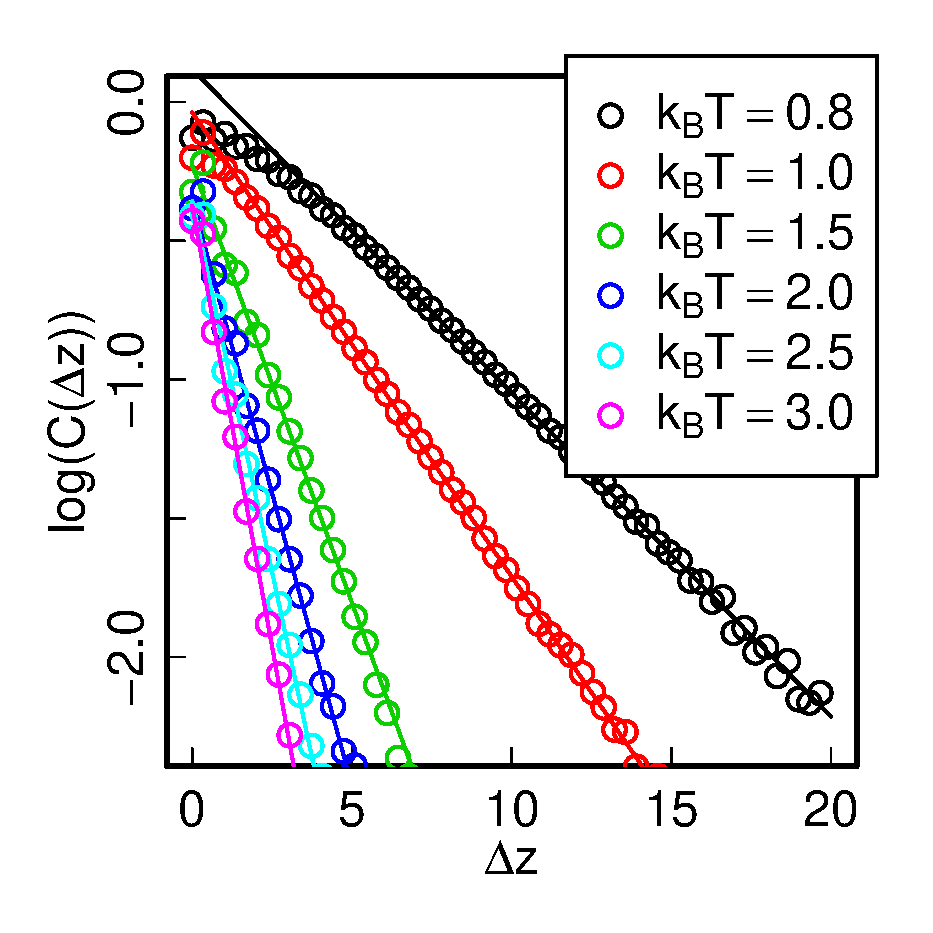
\includegraphics[width=\textwidth]{Images/distCor_50}
	\caption{$\rho = 0.50$}
\end{subfigure}
\begin{subfigure}[t]{0.32\textwidth}
	\centering
	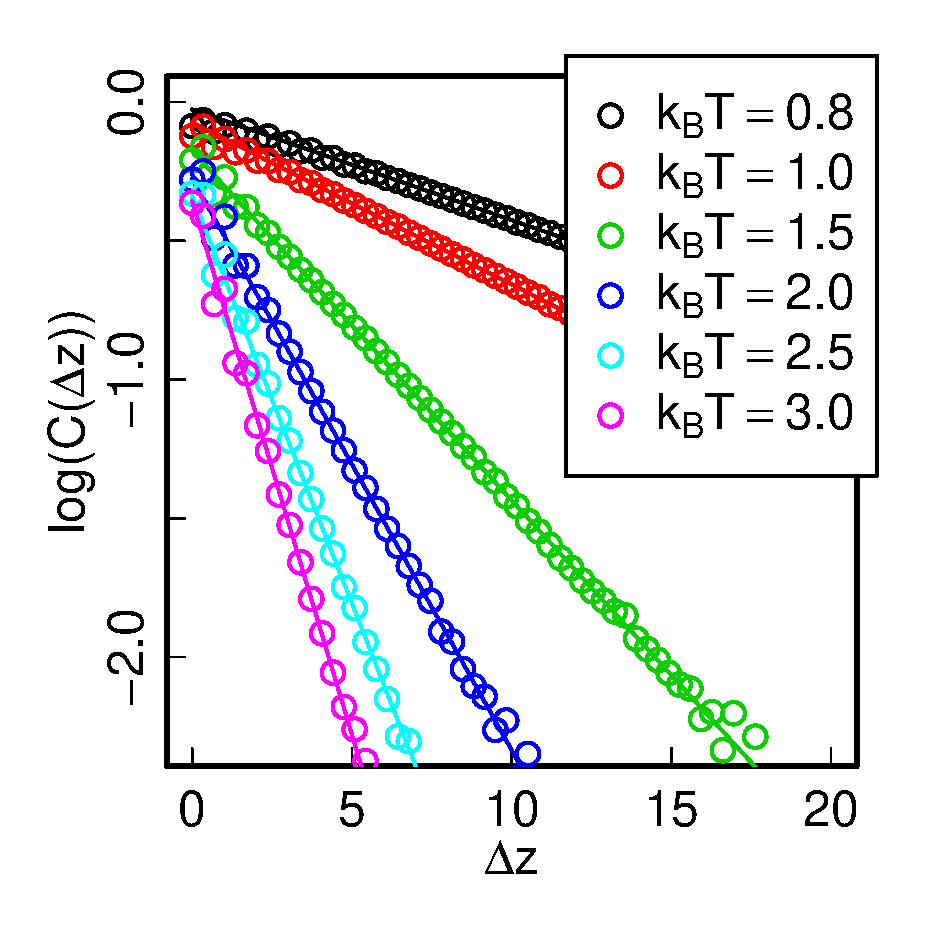
\includegraphics[width=\textwidth]{Images/distCor_75}
	\caption{$\rho = 0.75$}
\end{subfigure}
	\captionsetup{justification=centering, width=0.9\columnwidth}
	\caption{Orientation correlation as function of distance defined by eq.~\eqref{eq:distance_correlation} for Monte-Carlo simulations in the log-linear scale. The points are calculated for simulations with $N = 6400$ particles and the results are average over $200$ samples as described in sec.~\ref{subsec:simulation_details}. Lines are obtained by linear approximation of the results in range $0.01 < C(\Delta z) < 0.45$.}
	\label{fig:dist_corr_eq}
\end{figure}

We could now write $C(\Delta z)$ as
\begin{equation}
	\label{eq:slopes_def}
	C(\Delta z) \propto \exp^{A(k_BT, \rho) \Delta z}
\end{equation}
where $A$ is a function of system density and $k_BT$. If we look at the dependence of $A$ on the $k_BT$ for different system densities, we obtain the results shown at the Figure \ref{fig:dist_corr_eq_slopes}. For the high density $\rho = 0.75$ the \textcolor{red}{coefficient A} exhibits linear behaviour over all range of $k_BT$, while for the lower values of density the dependence consists of two linear regimes, with the transition occurring in the vicinity of $k_BT = 1.5$. On the Figure \ref{fig:dist_corr_eq_slopes} the dotted lines are the linear approximation in the range $k_BT \in (0.6, 1.5]$ while the solid lines show the approximation in range $k_BT \in (1.5, 3]$.

\begin{figure}[h]
\centering
\begin{subfigure}[t]{0.49\textwidth}
	\centering
	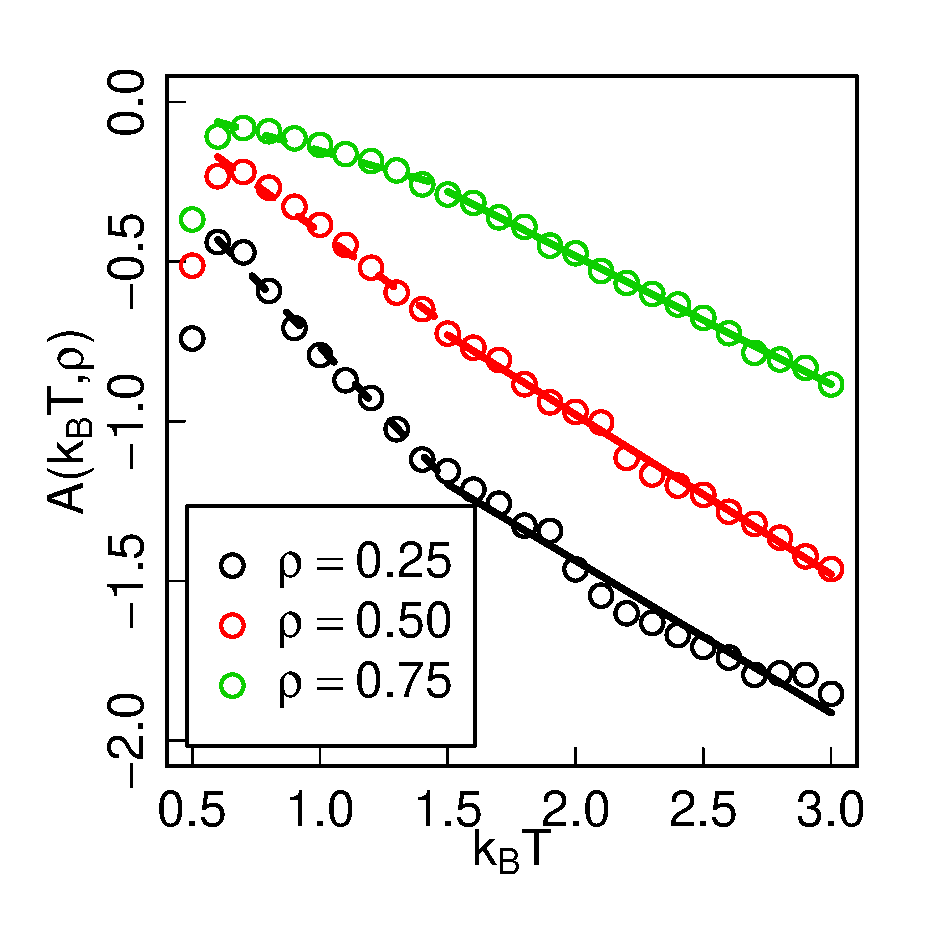
\includegraphics[width=\textwidth]{Images/distCorSlopes}
\end{subfigure}
	\captionsetup{justification=centering, width=0.9\columnwidth}
	\caption{$A(k_BT)$ as defined in \eqref{eq:slopes_def}. The points are the observed experimentally values of $A$ for different densities, and the lines are the linear approximation. The dotted lines are the linear approximation in the range $k_BT \in (0.6, 1.5]$ while the solid lines show the approximation in range $k_BT \in (1.5, 3]$.}
	\label{fig:dist_corr_eq_slopes}
\end{figure}

Defining ``chain'' we can distinguish three cases for the separation distance $d$. Firs being $d \ll R$ where $R$ is particle radius. That way we effectively treat all particles as ``unchained''. Second case is when $D \leq d < 2 D$, in which the ``chained'' particles form a compact cluster. And the third case is $d \sim L$, where $L$ is system size, in which the ``chain'' breaks only if particles orientations are not co-aligned with $z$ axis and each other.

Assuming all particles non-interacting ($k_BT \gg 1$) and unchained ($d \ll R$), for any angle $\alpha$ defined in \eqref{eq:chains_definition} we can calculate theoretically probability distribution for the case of two particles being oriented within conical angle $\alpha$, out of the conical angle, and the case when only one of the articles oriented out of conical angle, whereas the other is within. \textcolor{red}{rewrite, add about calculations. Area of spherical cap}.

That being said, we analyse how close is the probability of different particle pair configurations to the high-temperature limit for different $k_BT$. The results are shown on the Figure \ref{fig:chain_prob_dist_01}. The probabilities accumulate all possible configurations relatively to $z$ axis (i.e. RR defines sum of probability to have both particles oriented ``right'' and to have them oriented ``left'').

\begin{figure}[h]
\centering
\begin{subfigure}[t]{0.32\textwidth}
	\centering
	\includegraphics[width=\textwidth]{Images/probs_25}
	\caption{$\rho = 0.25$}
\end{subfigure}
\begin{subfigure}[t]{0.32\textwidth}
	\centering
	\includegraphics[width=\textwidth]{Images/probs_50}
	\caption{$\rho = 0.50$}
\end{subfigure}
\begin{subfigure}[t]{0.32\textwidth}
	\centering
	\includegraphics[width=\textwidth]{Images/probs_75}
	\caption{$\rho = 0.75$}
\end{subfigure}
	\captionsetup{justification=centering, width=0.9\columnwidth}
	\caption{Probability of having pair of particles both have orientation within conical angle $\alpha$ and co-aligned (RR), counter-aligned (RL). One of particles have orientation within and the other out of conical angle $\alpha$ (RU) and both particles having orientation out of conical angle $\alpha$ (UU).}
	\label{fig:chain_prob_dist_01}
\end{figure}